\documentclass[12pt, aspectratio = 169]{beamer} % handout

\usepackage{amsmath} % Mathematics related packages
\usepackage{fontawesome} % 'fontawesome' font
\usepackage{ragged2e}
\usepackage{color}
\usepackage[round]{natbib}
\usepackage{tikz}

% For 'InkScape' integration
\usepackage{import}
\usepackage{xifthen}
\usepackage{pdfpages}
\usepackage{transparent}

\usetheme[]{metropolis}
\usecolortheme[]{wolverine}

\usefonttheme{serif}
\setbeamercovered{transparent = 0.5}

\setbeamertemplate{theorems}[numbered] % Enables Definitions, Theorems, etc. numbering

\definecolor{title-bg}{RGB}{240, 240, 240} 
\definecolor{title-fg}{RGB}{128, 113, 93}
\definecolor{my-red}{RGB}{254, 132, 135}
\definecolor{my-blue}{RGB}{59, 180, 252}
\definecolor{my-green}{RGB}{125, 221, 149}
\definecolor{titles}{RGB}{0, 0, 112}
% \setbeamercolor{frametitle}{fg = titles, bg = title-bg}

\setbeamertemplate{footline}{%
	\leavevmode%
	\hbox{%
		\begin{beamercolorbox}[wd = 0.800\textwidth, ht = 4ex, dp = 2ex, left]{}%
			\hspace{6pt} \texttt{geoENV 2022.\phantom{|}14${}^{\text{th}}$ International Conference on Geostatistics for Environmental Applications.\phantom{|}June 22, 2022.}
		\end{beamercolorbox}%
		\begin{beamercolorbox}[wd = 0.120\textwidth, ht = 4ex, dp = 2ex, center]{}%
			\raisebox{-1pt}{\insertslidenavigationsymbol~\insertsectionnavigationsymbol}
		\end{beamercolorbox}%
		\begin{beamercolorbox}[wd = 0.080\textwidth, ht = 4ex, dp = 2ex, center]{}%
			\texttt{\insertframenumber~/~\inserttotalframenumber}
		\end{beamercolorbox}%
	}%
}%

% Personal Information
\author{André Victor Ribeiro Amaral \\ \href{mailto:andre.ribeiroamaral@kaust.edu.sa}{andre.ribeiroamaral@kaust.edu.sa}}

\begin{document}
	\AtBeginSection{}
	\metroset{block = fill}
	
	
	{
		\usebackgroundtemplate{
			\hspace{6pt}
			\includegraphics[width=0.35\textwidth]{Images/KAUST_logo.png}
			\hspace{230pt}
			\raisebox{5pt}{\includegraphics[width=0.15\textwidth]{Images/geoENV2022_logo.png}}
		}

		\begin{frame}[t]
			\centering
			\vspace{42pt}
			\textbf{{\large \usebeamercolor[fg]{frametitle} Spatio-temporal Point Process Compartment Modeling for Infectious Diseases}} \\
			\vspace{18pt}
			{\normalsize André V.\hspace{-1pt} Ribeiro\hspace{-1pt} Amaral\hspace{1pt}${}^{\star}$}\\
			{\scriptsize\texttt{\href{mailto:andre.ribeiroamaral@kaust.edu.sa}{andre.ribeiroamaral@kaust.edu.sa}}} \\
			\vspace{18pt}
			{\small King Abdullah University of Science and Technology}\\
			{\small Geospatial Statistics and Health Surveillance Research Group} \\
			\vspace{10pt}
			\begin{flushleft} {${}^{\star}$\hspace{1pt}\scriptsize Joint work with Jonatan A. González and Paula Moraga.}\end{flushleft}
		\end{frame}
	}
	
%	\begin{frame}[t]
%		\frametitle{Agenda}
%		\tableofcontents
%	\end{frame}
	
	\begin{frame}[t]
		\frametitle{Introduction}
		\justifying
		
		%One common approach to describe an epidemic dynamics consists of splitting the	population into compartments and modeling the rates, giving the parameters, that describe how an individual goes from one compartment to another.\vspace{-3pt}
		\begin{figure}[!ht]
			\centering
			\includegraphics[width = 1\textwidth]{Images/SIR_image.jpeg}\vspace{-6pt}
			\caption{\justifying Representation of susceptible (blue), infected (red), and recovered (green) individuals distributed in space at a given time point $t$.}
			\label{fig:SIRimage}
		\end{figure}
		
	\end{frame}

	\begin{frame}[t]
		\frametitle{Objective}
		\justifying
		
		We are also interested in modeling the infected individuals in space and time. And we will do this based on point pattern data observed at different time points.
		
		\pause
		
		In that way, our methodology addresses the epidemic spatio-temporal dynamics by modeling it in two steps
		
		\begin{enumerate}
			\justifying
			\item Fitting a temporal (compartment) model, and
			\item Using the previous step acquired information as the mean of a log-Gaussian Cox process for the point pattern representing the infected individuals in the studied region and time interval
		\end{enumerate}
		
	\end{frame}

	\begin{frame}[t]
		\frametitle{\texttt{SIR} modeling}
		\justifying
		
		The base-\texttt{SIR} model \citep{kermack1927contribution} is described by the following diagram\vspace{-12pt}
		\begin{figure}[!ht]
			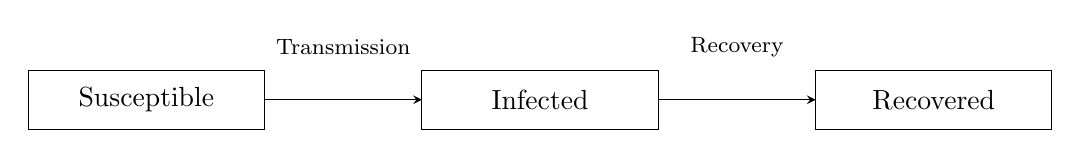
\begin{tikzpicture}
				\centering
				\draw[draw=black] (0, 0) rectangle ++(3, 0.75);
				\draw[draw=black] (5, 0) rectangle ++(3, 0.75);
				\draw[draw=black] (10, 0) rectangle ++(3, 0.75);
				\draw [-stealth](3, 0.375) -- (5, 0.375);
				\draw [-stealth](8, 0.375) -- (10, 0.375);
				\node[] at (1.5, 0.375) {Susceptible};
				\node[] at (6.5, 0.375) {Infected};
				\node[] at (11.5, 0.375) {Recovered};
				\node[] at (4, 1.05) {\footnotesize Transmission};
				\node[] at (9, 1.05) {\footnotesize Recovery};
			\end{tikzpicture}
		\end{figure}
		and it has the following assumptions
		\begin{enumerate}
			\item Homogeneous population with uniform mixing,
			\item Constant infectious and recovery rates over time, and
			\item Preserved population mass,
		\end{enumerate}

		\pause

		Many extensions of this model have been proposed (e.g., \texttt{SEIR}). Here, we will extend point (1.) of the base-\texttt{SIR} model to accommodate different age groups.

	\end{frame}

	\begin{frame}[t]
		\frametitle{\texttt{SIR} modeling}
		\justifying
		
		For $t \in \mathcal{T} \subseteq \mathbb{R}_{+}$, let $\texttt{S}_i(t)$, $\texttt{I}_i(t)$, and $\texttt{R}_i(t)$ denote the number of susceptible, infected, \hspace{-1pt}and recovered individuals, \hspace{-1pt}respectively,\hspace{-1pt} at time \hspace{-1pt}$t$ for age-group $i$. Then,
		\begin{align} \label{eq:SIRmodel}
			\frac{d\texttt{S}_i(t)}{dt} &= -\beta \texttt{S}_i(t) \sum_{\text{all}\,j}C_{ij}\cdot\frac{\texttt{I}_j(t)}{\texttt{N}_j} \\
			\frac{d\texttt{I}_i(t)}{dt} &= +\beta \texttt{S}_i(t) \sum_{\text{all}\,j}C_{ij}\cdot\frac{\texttt{I}_j(t)}{\texttt{N}_j} - \gamma \texttt{I}_i(t) \nonumber \\
			\frac{d\texttt{R}_i(t)}{dt} &= +\gamma \texttt{I}_i(t), \nonumber
		\end{align}
		such that $C_{ij}$ is a contact matrix, $\texttt{N}_i(t) = \texttt{N}_i$, $\forall t$, and $\beta, \gamma > 0$.
				
		\pause
				
		Model \eqref{eq:SIRmodel} will be solve it numerically. That is, given $(\texttt{S}_i(0), \texttt{I}_i(0), \texttt{R}_i(0))$, $\forall i$, we will define a solution at $\{t_k; k = 0, 1, \cdots, n\}$, such that $t_k \in \mathcal{T}$, $\forall k$.
		
	\end{frame}

	\begin{frame}[t]
		\frametitle{Point Process modeling}
		\justifying
		
		For the previous discretization  $\{t_k\}_k$, let $\xi(t_k)$ be a log-Gaussian Cox process driven by $\Lambda(\mathbf{u}; t_k)$.
		
		\pause
		
		In particular, we will define it as
		\begin{align} \label{eq:llambda}
			\Lambda(\mathbf{u}; t_k) = \mu(\mathbf{u}; t_k) \cdot \exp\{\zeta(\mathbf{u}; t_k)\}
		\end{align}
		where  $\zeta(\mathbf{u}; t_k)$ is a stationary Gaussian process with $\mathbb{E}(\zeta(\mathbf{u}; t_k)) = -\sigma^2/2$, $\forall k$ and $\mathbf{u}$, and $\text{Cov}(\zeta(\mathbf{u}_1; t_k), \zeta(\mathbf{u}_2; t_k)) = \sigma^2 \rho(h; t_k)$, such that  $\sigma^2$ is the variance and $h$ is the Euclidean distance between $\mathbf{u}_1$ and $\mathbf{u}_2$.
		
		As a remark, for specific choices of $\mu(\mathbf{u}; t_k)$, Model \eqref{eq:llambda} was previously discussed by \cite{diggle2006spatio}.
		
	\end{frame}

%	\begin{frame}[t]
%		\frametitle{Methodology}
%		\justifying
%		
%		In a nutshell, we are proposing a way to combine a SIR compartment model (with contact matrices information for different age groups), and a point process model.
%		
%		Such an approach allows us to take into account the temporal dynamics and understand the infectious individuals' spatial spread over time for each stratum of the population.
%		
%	\end{frame}

	\begin{frame}[t]
		\frametitle{Methodology}
		\justifying
		
		\begin{figure}[!ht]
			\centering
			\includegraphics[width = 1\textwidth]{Images/diagram.png}
			\caption{\justifying Two-step\hspace{-1pt} spatio-temporal\hspace{-1pt} modeling\hspace{-1pt} approach for infectious in all groups.}
			\label{fig:diagramST}
		\end{figure}
		
	\end{frame}

		\begin{frame}[t]
		\frametitle{Temporal modeling}
		\justifying
		
		Recall that, for a set of initial values  $(\texttt{S}_i(0), \texttt{I}_i(0), \texttt{R}_i(0))$, $\forall i$, and initial guesses for $\beta$ and $\gamma$, we can solve the system of ODEs for $\texttt{S}_i(t_k)$, $\texttt{I}_i(t_k)$, and $\texttt{R}_i(t_k)$ with some numerical method.
		
		For later reference, we will name these solutions $\texttt{S}_i^{\texttt{ODE}}(t_k)$, $\texttt{I}_i^{\texttt{ODE}}(t_k)$, and $\texttt{R}_i^{\texttt{ODE}}(t_k)$, respectively. 
		
		%Based on data given by a set of locations for each observed infected individuals, $\forall i$, namely $\{\xi_i(t_k)\}_k$ we will aggregate all locations over space in such a way that $\texttt{i}_i(t_k) = \#(\xi_i(t_k))$, $\forall i, k$. 
		
		%From such data, let's see how we can estimate the parameters from Model \eqref{eq:SIRmodel}. 
		
		%Once this is done, we can solve for $\texttt{S}_i(t_k)$, $\texttt{I}_i(t_k)$, and $\texttt{R}_i(t_k)$, $\forall i, k$, for inference and prediction.
		
	\end{frame}
	
	
	\begin{frame}[t]
		\frametitle{Temporal modeling}
		\justifying
		
		Now, suppose that we have obtained $\texttt{i}_i(t_k)$, $\forall i, k$.
		
		One way to model such data is assuming that they come from a certain probability distribution with mean given by the ODE solution $\texttt{I}_i^{\texttt{ODE}}(t_k)$, $\forall i, k$. In particular, we will assume
		\begin{align} \label{eq:InfNB}
			\texttt{I}_i(t_k) \sim \text{Negative Binomial}(\texttt{I}_{i}^{\texttt{ODE}}(t_k), \varphi),
		\end{align}
		such that $\varphi$ is the overdispersion parameter. This implies that $\mathbb{E}(\texttt{I}_i(t_k)) = \texttt{I}_{i}^{\texttt{ODE}}(t_k)$ and $\text{Var}(\texttt{I}_i(t_k)) = \texttt{I}_{i}^{\texttt{ODE}}(t_k)(1 + \texttt{I}_{i}^{\texttt{ODE}}(t_k) \cdot \varphi)$.
		
	\end{frame}
	
	\begin{frame}[t]
		\frametitle{Temporal modeling}
		\justifying
		
		For such an approach, notice that this is an iterative procedure. That is, 
		
		\begin{enumerate}
			\justifying
			\item Set initial values for $\beta$, $\gamma$, and $\varphi$.
			\item Solve Model \eqref{eq:SIRmodel} for $\texttt{S}_i(t_k)$, $\texttt{I}_i(t_k)$, and $\texttt{R}_i(t_k)$.
			\item Plug the $\texttt{I}_i^{\texttt{ODE}}(t_k)$ curve into the mean component of Model \eqref{eq:InfNB} to evaluate its likelihood function.
			\item Update $\beta$, $\gamma$, and $\varphi$, and get back to (2.) until reach convergence.
		\end{enumerate}
		
		Here, we adopt a Bayesian framework and use \texttt{RStan} \citep{rstanpackage} to estimate the posterior distribution of $\boldsymbol{\theta} = (\beta, \gamma, \varphi)^{\top}$.
		
	\end{frame}
	
	\begin{frame}[t]
		\frametitle{Spatio-temporal modeling}
		\justifying
		
		Given $\texttt{I}_i(t_k)$ curves, we will have the following model
		\begin{align*}
			\mathcal{N}_i(t_k)|\Lambda_i(\mathbf{u}; t_k) = \lambda_i(\mathbf{u}; t_k) \sim \text{Poisson}\left(\int_{\mathcal{U}}\lambda_i(\mathbf{u}; t_k)d\mathbf{u}\right),
		\end{align*}
		and the corresponding intensity functions will be described by
		\begin{align} \label{eq:Lambda}
			\Lambda_i(\mathbf{u}; t_k) &= \mu_i(\textbf{u}; t_k) \cdot \exp\{\zeta_i(\mathbf{u}; t_k)\},
		\end{align}
		such that
		\begin{align} \label{eq:muALT}
			\mu_i(\mathbf{u}; t_k) = \lambda_{0, i}(\mathbf{u}; t_k) \cdot \texttt{I}_i(t_k) \cdot \exp\{\omega_{1, i} \, x_{1, i}(\mathbf{u}; t_k) + \cdots + \omega_{p, i} \, x_{p, i}(\mathbf{u}; t_k)\},
		\end{align}
		where $\lambda_{0, i}(\mathbf{u}; t_k) \geq 0$, $\forall \mathbf{u}, k$, and  $\int_{\mathcal{U}}\lambda_{0, i}(\mathbf{u}; t_k) = 1$. $(x_{1, i}(\mathbf{u}; t_k), \cdots x_{p, i}(\mathbf{u}; t_k))$ is a vector of $p$ spatio-temporal covariates with coefficients $(\omega_{1, i}, \cdots, \omega_{p, i})^{\top}$.
	\end{frame}
		
	\begin{frame}[t]
		\frametitle{Spatio-temporal modeling}
		\justifying
		
		The final model is specified as follows
		\begin{align} \label{eq:modelSpatioTemporal}
			\mathcal{N}_i(t_k)|\Lambda_i(\mathbf{u}; t_k) = \lambda_i(\mathbf{u}; t_k) &\sim \text{Poisson}\left(\int_{\mathcal{U}}\lambda_i(\mathbf{u}; t_k)d\mathbf{u}\right), ~\forall i, k \\
			\Lambda_i(\mathbf{u}; t_k) &= \mu_i(\mathbf{u}; t_k) \cdot \exp\{\zeta_i({\mathbf{u}; t_k})\} \nonumber \\
			\mu_i(\mathbf{u}; t_k) &= \lambda_{0, i}(\mathbf{u}; t_k) \cdot \texttt{I}_i(t_k) \nonumber \\ 
			\zeta_i(\mathbf{u}; t_k | \boldsymbol{\eta}_i) &\sim \text{Gaussian Process} (\beta_{0, i}, \phi_i(h; t_k | \boldsymbol{\eta}_i)) \nonumber \\
			\boldsymbol{\eta}_i &\sim \text{priors}, \nonumber
		\end{align}
		such that $\phi_i(h; t_k | \boldsymbol{\eta}_i)$ is a covariance function that depends on the structure of $\zeta_i(\mathbf{u}; t_k)$, and $\boldsymbol{\eta}_i$ is the vector of parameters and hyperparameters.
		
		Model \eqref{eq:modelSpatioTemporal}  will be fitted using \texttt{R-INLA} \citep{rue2009approximate}. 
	\end{frame}
		
		\begin{frame}[t]
		\frametitle{Data Simulation}
		\justifying
		
		We consider as a study region an area of approx. 3 km${}^{2}$ in São Paulo, Brazil. For such a region, we divided people into three age groups: 0--19, 20--59, 60+.
		
		\begin{figure}[!ht]
			\centering\vspace{-3pt}
			\includegraphics[width = 0.95\textwidth]{Images/map.png}\vspace{-12pt}
			\caption{\justifying Studied region in  São Paulo (Brazil) with the overlapped grid for the estimated population and infected individuals' locations.}1
			\label{fig:map}
		\end{figure}
		
	\end{frame}
	
	\begin{frame}[t]
		\frametitle{Data Simulation}
		\justifying
		
		For a contact matrix and a vector of frequencies for people in each group, both previously estimated, we can, conditional on $\beta$, $\gamma$, and $\varphi$, simulate the $\texttt{I}_i(t_k)$ curves. We will do this for two scenarios, namely $\texttt{EP}$ (Early Peak) and $\texttt{FC}$ (Flat Curve).
		
		\begin{table}[!ht]
			\caption{\justifying SIR model parameters for the two scenarios, namely \texttt{EP} and \texttt{FC}, as we can see in Figure \ref{fig:simulatedSIR}.}
			\centering
			% \resizebox{\textwidth}{!}{%
				\begin{tabular}{c|c|c}
					& Scenario \texttt{EP} & Scenario \texttt{FC} \\ \hline
					$\beta$     & 0.04   &  0.0175 \\
					$\gamma$    & 0.2\phantom{0} &  0.1\phantom{000} \\
					1/$\varphi$  & 0.01   &  0.01\phantom{00}
				\end{tabular}%
				% }
			\label{tab:parametersSIR}
		\end{table}
		
	\end{frame}
	
	\begin{frame}[t]
		\frametitle{Data Simulation}
		\justifying
		
		Then, based on Table \ref{tab:parametersSIR}, we can generate curves for the two scenarios.
		
		\begin{figure}[!ht]
			\centering
			\includegraphics[width = 1\textwidth]{Images/SIRplots.png}\vspace{-6pt}
			\caption{\justifying Simulated $\texttt{I}_i(t_k)$ curves, for all age groups 1, 2, and 3 (which corresponds to ages 0--19, 20--59, 60+, respectively). Scenarios \texttt{EP} (left) and \texttt{FC} (right).}
			\label{fig:simulatedSIR}
		\end{figure}
		
	\end{frame}
	
	\begin{frame}[t]
		\frametitle{Data Simulation}
		\justifying
		
		Once we have simulated the $\texttt{I}_i(t_k)$ curves, $\forall i$, the true generated intensity functions will be sampled from the following model 
		\begin{align*}
			\Lambda_i(\mathbf{u}; t_k) &= \lambda_{0, i}(\mathbf{u}; t_k) \cdot \texttt{I}_i(t_k) \cdot \exp\{\zeta_i(\mathbf{u}; t_k)\}, \text{ for each } i \text{ and } k = 0, 1, 2, \cdots\hspace{-1pt}, 99,
		\end{align*}
		such that $\lambda_{0, i}(\mathbf{u}; t_k)$ is the normalized populational grid and  $\zeta_i(\mathbf{u}; t_k)$  is defined as before.
		
	\end{frame}

		\begin{frame}[t]
		\frametitle{Model Fitting}
		\justifying
		
		Given the data, we can fit a null model ($\mathcal{M}_0$) and an alternative model ($\mathcal{M}_1$). In particular, for $\xi_{i}(t_k)$ modeled as follows
		\begin{align*}
			\mathcal{N}_i(t_k)|\Lambda_i(\mathbf{u}; t_k) = \lambda_i(\mathbf{u}; t_k) \sim \text{Poisson}\left(\int_{\mathcal{U}}\lambda_i(\mathbf{u}; t_k)d\mathbf{u}\right),
		\end{align*}
		the null model ($\mathcal{M}_0$) will be given by
		\begin{align*}
			\Lambda_i(\mathbf{u}; t_k) &= \exp\{\omega_{0, i} + \zeta_i(\mathbf{u}; t_k)\}, 
		\end{align*}
		such that $\omega_{0, i}$ is an unknown intercept, and the alternative model ($\mathcal{M}_1$) will be given by
		\begin{align*}
			\Lambda_i(\mathbf{u}; t_k) &= \mu_{i}(\mathbf{u}; t_k) \cdot \exp\{\zeta_i(\mathbf{u}; t_k)\}, 
		\end{align*}
		where $\mu_{i}(\mathbf{u}; t_k)$ is defined as in Equation \eqref{eq:muALT}. $\zeta_i(\mathbf{u}; t_k)$ is defined accordingly.
	\end{frame}
	
%	\begin{frame}[t]
%		\frametitle{Implementation and Results}
%		\justifying
%		
%		Estimated parameters for both scenarios, namely \texttt{EP} and \texttt{FC}, are shown below.	
%		\begin{table}[!ht]
%			\caption{\justifying Estimated SIR model parameters (and 95\% equal-tail credible interval) for the two scenarios, namely \texttt{EP} and \texttt{FC}. Models were fitted with data up to $t_k = 49$.}\vspace{-18pt}
%			\centering
%			\resizebox{\textwidth}{!}{%
%				\begin{tabular}{c|c|c|c|c}
%					& Scenario & True value & Posterior mean & 95\% equal-tail credible interval \\ \hline
%					$\beta$ & \texttt{EP} &       0.04\phantom{00} & 0.0400 & (0.0399, 0.0402) \\ 
%					$\gamma$ & \texttt{EP}&       0.2\phantom{000} & 0.1998 & (0.1972, 0.2024) \\ 
%					$1/\varphi$  & \texttt{EP} &  0.01\phantom{00} & 0.0095 & (0.0070, 0.0132) \\ 
%					$\beta$ & \texttt{FC} &       0.0175\phantom{} & 0.0173 & (0.0170, 0.0176) \\ 
%					$\gamma$ & \texttt{FC} &      0.1\phantom{000} & 0.0964 & (0.0912, 0.1013) \\ 
%					$1/\varphi$  & \texttt{FC} &  0.01\phantom{00} & 0.0091 & (0.0067, 0.0131) \\ 
%				\end{tabular}%
%			}
%			\label{tab:estimatedSIRparameters}
%		\end{table}
%		
%	\end{frame}
	
	\begin{frame}[t]
		\frametitle{Implementation and Results}
		\justifying
		\begin{figure}[!ht]
			\centering
			\includegraphics[width = 1\textwidth]{Images/estimated_SIR_curves_one.png}
			\caption{\justifying Estimated $\texttt{I}_i(t_k)$ curves for the age group 20--59 in the two scenarios, namely \texttt{EP} (left) and \texttt{FC} (right). 95\% prediction intervals are also presented. \textbf{Models were fitted with data up to $t_{49}$} (vertical dashed line).}
			\label{fig:estimatedSIRonegroup}
		\end{figure}
		
	\end{frame}
	
	\begin{frame}[t]
		\frametitle{Implementation and Results}
		\justifying
		
		Based on a point estimate for $\texttt{I}_i(t_k)$, as we have just obtained, now we can employ our modeling approach in space-time; that is, as before
		\begin{align*}
			\mathcal{N}_i(t_k)|\Lambda_i(\mathbf{u}; t_k) = \lambda_i(\mathbf{u}; t_k) &\sim \text{Poisson}\left(\int_{\mathcal{U}}\lambda_i(\mathbf{u}; t_k)d\mathbf{u}\right), ~\forall i, k \\
			\Lambda_i(\mathbf{u}; t_k) &= \mu_i(\mathbf{u}; t_k) \cdot \exp\{\zeta_i({\mathbf{u}; t_k})\} \nonumber \\
			\mu_i(\mathbf{u}; t_k) &= \lambda_{0, i}(\mathbf{u}; t_k) \cdot \texttt{I}_i(t_k) \nonumber \\ 
			\zeta_i(\mathbf{u}; t_k | \boldsymbol{\eta}_i) &\sim \text{Gaussian Process} (\beta_{0, i}, \phi_i(h; t_k | \boldsymbol{\eta}_i)) \nonumber \\
			\boldsymbol{\eta}_i &\sim \text{priors}, \nonumber
		\end{align*}
		
		%For the inference and prediction steps, we will use the same grid as in the Figure \ref{fig:map}. 
		
		%In particular, we will compare the null model ($\mathcal{M}_0$) and the alternative model ($\mathcal{M}_1$).
		
		And all fitting procedure will be performed based on data observed up to $t_{49}$.
		
	\end{frame}

	\begin{frame}[t]
		\frametitle{Model Assessment}
		\justifying
		
		To compare the models, we will compute the Mean Arctangent Absolute Percentage Error (MAAPE) \citep{kim2016new}. For each group $i$ and at $t_k$, 
		\begin{align*}
			\text{MAAPE}_{i, k} = \frac{1}{J} \sum_{j = 1}^{J} \arctan\left(\left|\frac{(f_{i, j, k} - \hat{f}_{i, j, k})}{f_{i, j, k}}\right|\right).
		\end{align*}
		such that $J$ is the total number of cells, and $f_{i, j, k}$ and $\hat{f}_{i, j, k}$ correspond to the true and predicted number of infectious in group $i$, cell $c_j$, and at $t_k$, respectively.
		
	\end{frame}
	
	\begin{frame}[t]
		\frametitle{Model Assessment}
		\justifying
		
		MAAPE for null and alternative models for $\texttt{EP}$ (left) and $\texttt{FC}$ (right) scenarios.\vspace{-3pt}
		\begin{figure}[!ht]
			\centering
			\includegraphics[width = 1\textwidth]{Images/computed_errors.png}\vspace{-6pt}
			\caption{\justifying Computed MAAPEs for groups 1, 2, and 3 (0--19, 20--59, 60+,  respectively). Models were fitted with data up to $t_{49}$ (vertical solid line).}
			\label{fig:computederrors}
		\end{figure}
		
	\end{frame}
	
	\begin{frame}[t]
		\frametitle{Discussion}
		\justifying
		
		We proposed a two-step framework for modeling data on the infectious locations and times as follows: first, using a compartment model;  and second, incorporating such an information to a  log-Gaussian Cox process model.
		
		\pause
		
		By doing this, provided the temporal model in the first step is well specified,	the spatio-temporal modeling will produce reasonably good predictions. 
		
		\pause
		
		If SIR assumptions do not hold, step one can be modified to different statistical models. In this case, long-term predictions might not be as good, though.
		
		\pause
		
		Also, we used the exact locations and times of infected individuals. These data may be challenging to obtain. However, if good quality data is available, we think the proposed model can help understand infectious disease spreading.
	
	\end{frame}
		
	\begin{frame}[t] % allowframebreaks
		\frametitle{References}
		\justifying
		\footnotesize
		%\nocite{hernandez2020evaluating}
		\bibliographystyle{apalike}
		\bibliography{References/References}
	\end{frame}

	\begin{frame}[t]
			\frametitle{Omitted Details}
			\justifying
			
			From Equation \eqref{eq:Lambda}, $\zeta_i(\mathbf{u}; t_k)$ can be defined in different ways. However, throughout this presentation, we considered the following
			\begin{align} \label{eq:zeta}
					\zeta_i(\mathbf{u}; t_k) = \beta_{0, i} + \vartheta_i(\mathbf{u}; t_k) + \upsilon_i(t_k) + \varepsilon_i(\mathbf{u}; t_k), ~\forall i,
				\end{align}
			where $\vartheta_i$ is a zero-mean Gaussian process with covariance function $\sigma_i^2 \rho(h; t_k)$, such that $\rho(h; t_k)$ will be given by the Matérn model, 
			\begin{align*}
					\upsilon_i(t_k) &= \varrho_i(t_k),  \text{ for } k = 0 \\
					\upsilon_i(t_k) &= \alpha_i \upsilon_i(t_{k-1}) + \varrho_i(t_k), \text{ for } k = 1, \cdots, n,
				\end{align*}
			where $|\alpha_i| < 1$, $\forall i$, and $\varrho_i(t_k)$ is a zero-mean temporally independent Gaussian process with variance $\sigma_{i, \varrho}^2$, and $\varepsilon_i(\mathbf{u}; t_k)$ is a zero-mean temporally independent Gaussian process with variance $\sigma^{2}_{i, \varepsilon}$.  In that case, $\mathbb{E}(\zeta_i(\mathbf{u}; t_k)) = \beta_{0, i}$.
		\end{frame}
	
\end{document}